Advances in sequencing technologies have enabled novel insights into microbial niche differentiation, from analyzing environmental samples, to understanding human diseases and informing dietary studies.  However, identifying the microbial taxa that differentiate these samples can be challenging. These issues stem from the compositional nature of 16S \gls{rrna} gene data (or, more generally, taxon or functional gene data), which changes in the relative abundance of one taxon influence the apparent abundance of the others.  Here we acknowledge that inferring properties of individual bacteria is a difficult problem, and instead introduce the concept of balances to infer meaningful properties of sub-communities, rather than properties of individual species.  We show that balances can yield insights about niche differentiation across multiple microbial environments including soil environments and lung sputum. These techniques have the potential to reshape how we carry out future ecological analyses aimed at revealing differences in relative taxonomic abundance across different samples.
\section{Introduction}
The ultimate goal for many microbial ecologists is to fully characterize niches of microbial organisms and understand interactions among taxa.  An understanding of how microbial communities are affected by environmental conditions could yield insights into microbial interactions and their role in macro-ecological processes, such as nitrogen fixation \cite{nitrogen_fixation} and acidification \cite{acidification}. But despite the extraordinary increase in available data brought about by advances in DNA sequencing, characterizing niche differentiation in microbes remains an outstanding problem, partly due to the difficulty of correctly interpreting compositional data.  Broadly speaking, a compositional dataset is represented by relative abundances, or proportions that individually carry no meaning on the absolute abundance of a specific feature (i.e. 20\% of 100 and 20\% of 10,000 are very different absolute abundances).  The constraints associated with compositional data are well known, but unfortunately often neglected in microbial ecology, leading to conflicting interpretations and irreproducible analyses \cite{gloor_epi, fodor_coda} .\par
\begin{figure}[H]
        \centering
        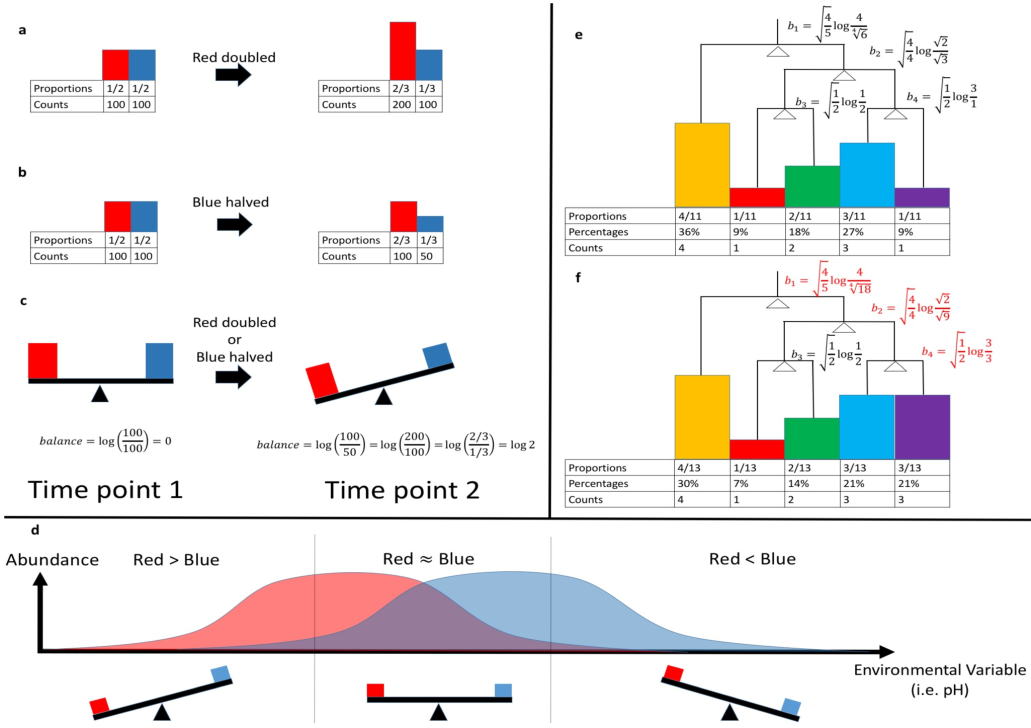
\includegraphics[width=1\textwidth]{ch3/Figure1.pdf}
        \caption[An explanation of balances and how to interpret them.]
        {An explanation of balances and how to interpret them. (a, b) A hypothetical scenario where 2 samples of 2 proportions could explain two different scenarios in the environment.  The balance between these 2 proportions is consistent for both scenarios.  (c) The balance of Red and Blue species abundances.  (d) balances of Red and Blue individuals across an environmental variable.  (e, f) The comparison of proportions and balances of two environments in the scenario where the Purple Orange population (i.e. the most right bin) triples. The balances were calculated using the groupings specified by the tree.\index{SanDiego8}}
        \label{figc1}
\end{figure}
We illustrate an example of this problem in Figure \ref{figc1}.  In this scenario, there are two species, “Red” and “Blue”. At the first time point, there are 100 Red individuals and 100 Blue individuals (Figure \ref{figc1}a). At the next time point, the number of Red individuals doubles, yielding 200 Red individuals, and the proportion of Red and Blue individuals becomes 2/3 and 1/3, respectively (Figure \ref{figc1}b). Suppose that we do not know the true total number of individuals in the given environment, and can only make inferences about the observed proportions -- a common scenario in microbial ecology, where absolute quantification is rarely performed.  In Figure \ref{figc1}b, the community has the exact same proportions at Time 1 and Time 2 as Figure \ref{figc1}a; however, instead of the Red individuals doubling at the second time point, the number of Blue individuals is halved (Figure \ref{figc1}c).\par
This is the problem with compositionality -- based on proportions alone, it is impossible to determine whether the growth or decline of any individual species has truly occurred \cite{Lovell_David_Muller_Warren_Taylor_Jennifer_Zwart_Alec_Helliwell2010-na}, and the inherent feature of one change in abundance driving abundance changes in another species violates assumptions of independence.  Analyses that rely on such assumptions, as many statistical approaches do, are thus prone to misinterpretation. For example, traditional correlation metrics such as Pearson and Spearman can be misleading when estimating microbe-microbe correlations \cite{sparcc, proportionality, spiec_easi, weiss_normalization}.  As a result, it becomes a major challenge to specify types of interactions between microbes, such as parasitism, competition, predation or mutualism, as shown in correlations studies in oral, fecal and vaginal samples from the Human Microbiome Project \cite{faust_microbial_interactions} \cite{sparcc}.  Even more advanced correlation-detection techniques such as SparCC \cite{sparcc} and SPIEC-EASI \cite{spiec_easi}, struggle with this, and typically require additional assumptions such as sparse \gls{otu} correlations (i.e. few \gls{otu}s are actually correlated with each other).  Furthermore, interpreting the resulting network is a major challenge, making it difficult to differentiate between true ecological relationships and random processes \cite{faust_microbial_interactions}.\par
The compositionality problem is also problematic for statistically detecting differentially abundant microbes across environments or between groups — consequently, it is a major barrier to reliably drawing conclusions about realized microbial niches using community sequencing data. Conventional statistical tools such as t-test and Mann-Whitney can incorrectly identify nearly 100\% of the taxa present in samples to be significantly different across environments (Figure S1), and univariate tests such as t-tests and ZIG \cite{metagenomeSeq} have been shown to mislabel microbes as significantly different across sample groups up to 60\% of the time \cite{ancom}. More advanced tools for differential abundance detection such as (\gls{ancom}) \cite{ancom}, are typically designed to control for false-positives and reliably detect differentially abundant species, but require multiple assumptions (i.e. the number of changing microbes across environments is small) and may require complex parameter tuning. To help overcome these issues of compositionality, we explore using the concept of balances, by moving away from inferring changes of individual species to instead inferring changes of microbial sub-communities to study niche differentiation of microbial communities.\par
\section{Concept}
Balances were first introduced as an exploratory technique in geology \cite{groups_of_parts, coda_dendrogram}. Fundamentally, they overcome the prhoblem of inferring changes in abundance from compositional data by sidestepping it, and instead inferring changes in the balance between particular subsets of the community. To understand the concept, let us revisit the scenario in Figure \ref{figc1}a and \ref{figc1}b.  Instead of examining proportion changes, we can investigate the balance between Red and Blue individuals by taking the log ratio of Red and Blue counts (Figure \ref{figc1}c).  By looking at the balance of these two species, we avoid incorrectly attempting to infer absolute increases or decreases in their abundances.  Instead, we can focus on the balance of the Red and Blue individuals, and directly infer the transition of dominance between these species.\par
These balances can also be useful for understanding species distributions across different covariates — a key proximate goal of microbial ecology, and one that is both crucial to the larger goal of niche characterization and heavily impacted by problems inherent in compositionality.  In Figure \ref{figc1}d, the Red individuals tend to exist in the low pH end of the spectrum, while the Blue individuals tend to exist in the high pH end of the spectrum.  A single balance can capture information about the transition from a high relative abundance of Red individuals in low pH environments to a high relative abundance of Blue individuals in high pH environments.  In low pH environments, the balance is positive, since there are proportionally more Red individuals than Blue individuals.  When the Red and Blue individuals are present in roughly equal proportions, the balance is roughly zero, representing a turning point, transitioning from a Red dominated community to a Blue dominated community.  As the pH increases, the balances become increasingly negative, since there are more Blue individuals than Red individuals. This balance effectively encodes for the niche separation of Red and Blue individuals across the pH gradient. \par
This idea of balances can be extended to multiple dimensions — and more than two taxa — using bifurcating trees.  A bifurcating tree can be built relating microbial taxa to each other using any criterion, and balances can be calculated on the internal nodes of the tree from the geometric means of the corresponding sub-trees. The appropriate criterion to build a tree depends on the question at hand.  A phylogenetic tree could be used to investigate evolutionary relationships of microbes \cite{Silverman2018-ql, Washburne2017-up}, or hierarchical clustering of environmental variables could be used to explore environmental niches of microbes.  To gain more intuition about this, consider Figure \ref{figc1}e, in which there are five species and 11 individuals. The four balances (internal nodes in the tree) are calculated by taking the log ratio of geometric means of sub-trees, also known as the isometric log ratio (\gls{ilr}) transform.  The full equation to calculate balances for a single sample is as follows,
\begin{equation}
b_{i}=\sqrt{\frac{\left| i_{L}\right| \left| i_{R}\right|}{\left| i_{L}\right|+ \left| i_{R}\right|}}log \frac{g(i_{L})}{g(i_{R})}
\end{equation}
where $b_{i}$ is the balance of the at internal node i ,  $i_{L}$, is the set of all species proportions contained in the left sub-tree at internal node i, $i_{R}$,  is the set of all species proportions contained in the right subtree at the internal node  i, g(x),  is the geometric mean of all of the proportions contained in vector $x$, $ \left| i_{R}\right|$,  is the number of species contained in  $i_{R}$ , and  $ \left| i_{L}\right|$ is the number of species contained in $ i_{L}$ (see Materials and Materials for more details). Following this equation, in Figure \ref{figc1}f  $b_{1}$ is calculated by taking the log ratio of the Yellow species and the geometric mean of the Red, Green, Blue, and Purple species.  \par
 It's also important to note that the some of the balances don't impact each other.  For instance, the changes in b4 do not impact the changes in b3, just because these balances don't share any common tips.  This is crucial, because this property allows us to ignore some of the variance of the balances towards the tips of the tree, and focus on the balances closer to the root of the tree.  These balances toward the root of tree capture the most information, since they contain a significant proportion of tree tips.  As a result, these high level balances have the potential to explain large shifts in these microbial communities.  The choice of the tree can allow for analysts to embed prior knowledge into the structure of the tree to test for these large community shifts.\par
 Here, we will discuss two studies from which novel insights were gained from this application.  While there are many compositionally aware tools available that are designed to identify microbial interactions and abundance fluctuations, we will refrain from benchmarking balances against these tools, as balances answer a conceptually different question.  These analyses are not restricted to analyzing ratios of individual \gls{otu}s and can be easily extended to analyze ratios of subcommunities.  \par
\section{ Results}
 \subsection{Case Study \#1 – Balances of pH-driven subcommunities in soils}
 In this study \cite{soil_pyro}, 88 soil samples were collected from North and South America, along with many edaphic measurements.  The study reported that there was a strong correlation between pH and species richness, suggesting that pH was a strong driver behind fluctuations in soil microbial communities. Acidobacteria were found to be negatively correlated with pH and Actinobacteria and Bacteroidetes to be positively correlated with pH, while Alpha/Beta/Gammaproteobacteria were not correlated with pH at all.  These correlation analyses are a little misleading, since the pH was correlated with each of the phyla independently.  The problem with this approach is that it does not account for all of the other phyla: similar to the argument made in Figure \ref{figc1}b, the change in a single phylum could also be explained by correlated changes in all of the other phyla.  Here, the negative correlation between Acidobacteria and pH could also be caused by the positive correlation between Bacteroidetes and pH.  Additionally, we cannot determine whether the Alpha/Beta/Gammaproteobacteria are correlated with pH or not.  Another possibility is that these three phyla could be positively correlated with pH, while Acidobacteria is not correlated with pH.  However, Bacteroidetes may be so strongly correlated with pH that Acidobacteria appears to be negatively correlated with pH, and the other three phyla not correlated with pH at all.  This scenario is one of the infinite possible underlying relationships that can explain these observed correlations. \par
 \begin{figure}[H]
        \centering
        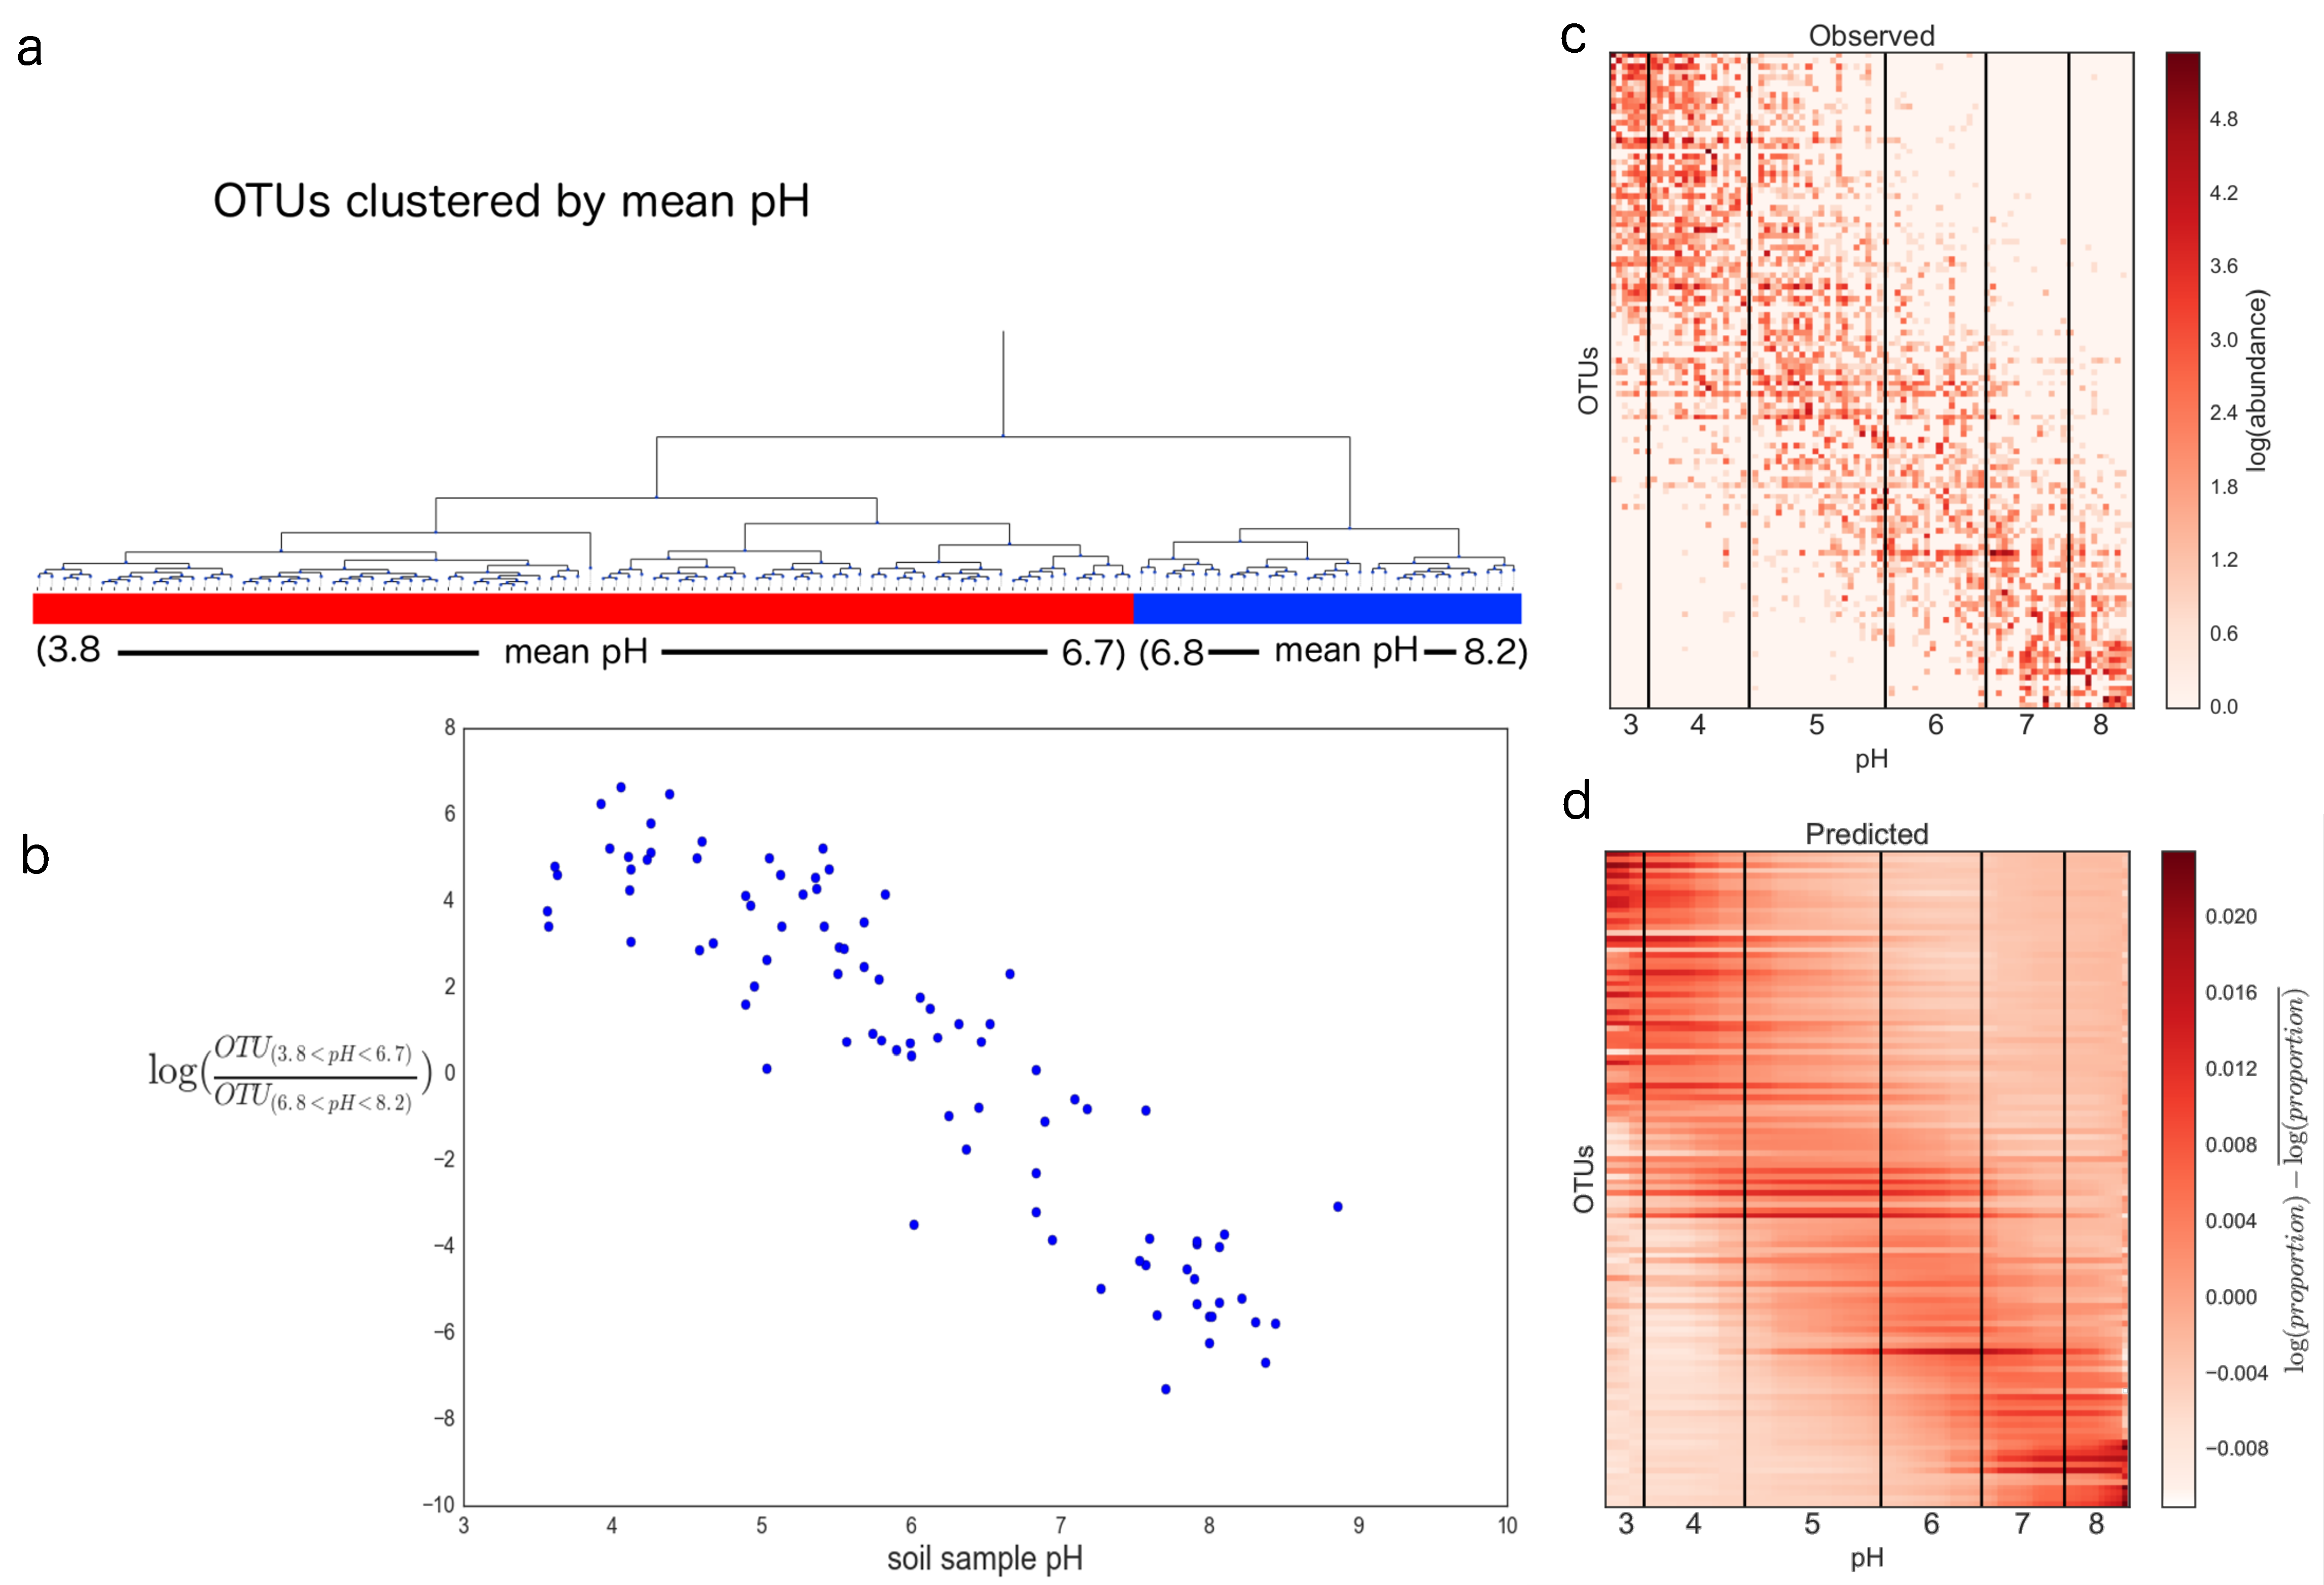
\includegraphics[width=1\textwidth]{ch3/Figure2.pdf}
        \caption[The application of balances on a soil microbial dataset to identify
          microbial partitioning with respect to pH.]
        {The application of balances on a soil microbial dataset to identify microbial partitioning with respect to pH.(a) Hierarchical clustering of closed ref \gls{otu}s based on mean pH. (b) The balance of low pH associated organisms (3.8 $<$ mean pH $<$ 6.7) and high pH associated organisms (6.8 $<$ mean pH $<$ 8.2). (c) Observed \gls{otu} counts sorted by pH. (d) Predicted \gls{otu} proportions from ordinary least squares linear regression on balances sorted by pH. The coefficient of determination was 35\%, showing that 35\% of the variation in the microbial community abundance data can be predicted by pH alone.\index{SanDiego8}}
        \label{figc2}
 \end{figure}
 At a first glance, uncovering the true correlations correctly appears to be a hopeless cause.  This is where balances become useful.  Rather than attempting to correlate individual phyla against pH, we will group \gls{otu}s together according to their difference in mean pH (Figure \ref{figc2}a), and investigate how these balances of groups changes with respect to pH (See Materials and Methods on hierarchical clustering).  This circumvents the dependence issue noted previously.  We do not need to worry about subgroups within the left and right subtrees of a balance to be influencing each other, due to the independence property shown in Figure \ref{figc1}ef.  \par
 The balance concept proves to be a very powerful technique for investigating how these groups of organisms change relative to each other as pH increases.  Recall the cartoon example in Figure \ref{figc1}d.  If there are two distinct unimodal species distributions, the balance pivots from being weighted by Red in low pH, to being weighted by Blue in high pH.  The exact same phenomenon is occurring here, except there are multiple species on the left end of the balance, and multiple species on the right end of the balance.\par
 As shown in Figure \ref{figc2}b, there is a well defined trend of low pH \gls{otu}s (3.8 $<$ mean pH $<$ 6.6) gradually being overtaken by high pH \gls{otu}s (6.7 $<$ mean pH $<$ 8.2) as the pH increases, forming a nice linear trend defined by the top balance in the tree shown in Figure \ref{figc2}a.  If we were to sort the samples by their mean pH, and the \gls{otu}s by their mean pH (Equation 3), a well defined band pattern appears.  Here, it is clear that \gls{otu}s with a mean pH less than 3 rarely have nonzero counts above 8.  Likewise, \gls{otu}s that have a mean pH more than 8 rarely have nonzero counts below 3.  If we were to tie in this band pattern in Figure \ref{figc2}c together with the balance vs pH trends shown in Figure \ref{figc2}b, we would obtain a very different interpretation from the original study.  \gls{otu}s tend to be observed in very specific pH ranges, but not commonly observed outside of these ranges.  This ties together with some concepts in niche theory - \gls{otu}s are more suited to live within a designated range of pHs.  And if they are placed outside of this pH range, they are outcompeted by other organisms who are more suited to live within the given pH range.  \par
 These patterns were completely missed when only looking at the phylum level in the original study.  In fact, based on the calculated mean pH values for each \gls{otu}s, it is observed that \gls{otu}s from all of the phyla mentioned in the study are widely distributed across the pH gradient (Supplemental Table 1).  As an extreme example, \gls{otu}s from the family Bradyrhizobiaceae were observed to be present in both ends of the spectrum, some present at pH values as low as 5.36, while others present at a pH as high as 6.75.  These are astronomical differences, considering
 that 95\% of the \gls{otu}s have a mean pH that falls between this range. This provides additional justification for building a tree based on mean pH, rather than bacterial phylogeny.\par
  Finally, these balances can be used to build predictive models.  Using ordinary least squares on the calculated balances, the entire microbial community profile can be predicted using pH alone with an $R^2$ of 0.35. This means that pH alone explains over 35\% of the total variation in entire soil microbial communities across North and South America. The resulting fit can be transformed back to proportions to yield the predicted proportions (Figure \ref{figc2}d).  From this heatmap, the key patterns are still retained, such as the band pattern apparent in Figure \ref{figc2}c. There are many regression techniques published that attempt to use microbial abundances to predict covariates, such as the post-mortem interval \cite{mammalian_corpse} or body mass index \cite{microbial_regression}. This approach is the first of its kind to attempt to address the reverse problem to predict entire microbial community distributions based on environmental variables. These predictions were enabled by the powerful fundamental properties of balances.\par
  \subsection{Case Study \#2 – Balances of pH-driven subcommunities in a lung sputum culture microcosm}
 In this study, lung sputum samples were collected from 16 cystic fibrosis (\gls{cf}) patients.  These sputum samples were then grown in a capillary tube culture system (Winogradsky Cystic Fibrosis system) that mimics the conditions of a lung bronchiole \cite{wincf}.  These samples were placed into separate tubes and the pH of the media was adjusted from 5 to 8.5 at intervals of 0.5 to determine how the microbial community changed with respect to pH.  After growth in the capillary tubes, the communities were assessed using 16S \gls{rrna} gene amplicon sequencing.\par
 One of the difficulties in this study was characterizing pathogenic bacteria.  Early on in this case study, the only significant finding discovered was that patients had different lung sputum microbiomes (Figure \ref{figc3}a). It was hypothesized that there was a subcommunity of low pH organisms and a subcommunity of high pH organisms that periodically appeared and disappeared in \gls{cf} lung sputum.  However, these changes could not be detected using available statistics, likely due to the compositionality problem.  Since the different \gls{cf} patients had idiosyncratic lung communities, they ended up having different \gls{otu}s responding across the laboratory pH gradient, yielding insufficient statistical power to detect changes in any given \gls{otu}.  As a result, when these lung sputum communities were placed into different media and studied, it was not clear exactly what organisms were a part of this low pH or high pH subcommunity.  \par
 Balances are a natural solution to this problem.  In addition to probing for similar patterns to those observed in the previous study, balances are well adapted as a transformation for standard statistical analyses.  Since Euclidean operations directly translate into perturbation and powering operations on proportions \cite{ilr, Pawlowsky-Glahn2015-qb}, many publicly available statistical tools can be applied to directly to balances.  For this study, we opted to use Linear Mixed Effects models to test for pH differences while simultaneously accounting for all of the differences between lung microbiomes across \gls{cf} patients.   Based on prior analyses with pH in soils, the tree was built using the exact same strategy (See Methods and Materials).   Significant balances testing for pH were determined with a p-value cutoff at 0.05 after Bonferroni correction.  \par
  \begin{figure}[H]
        \centering
        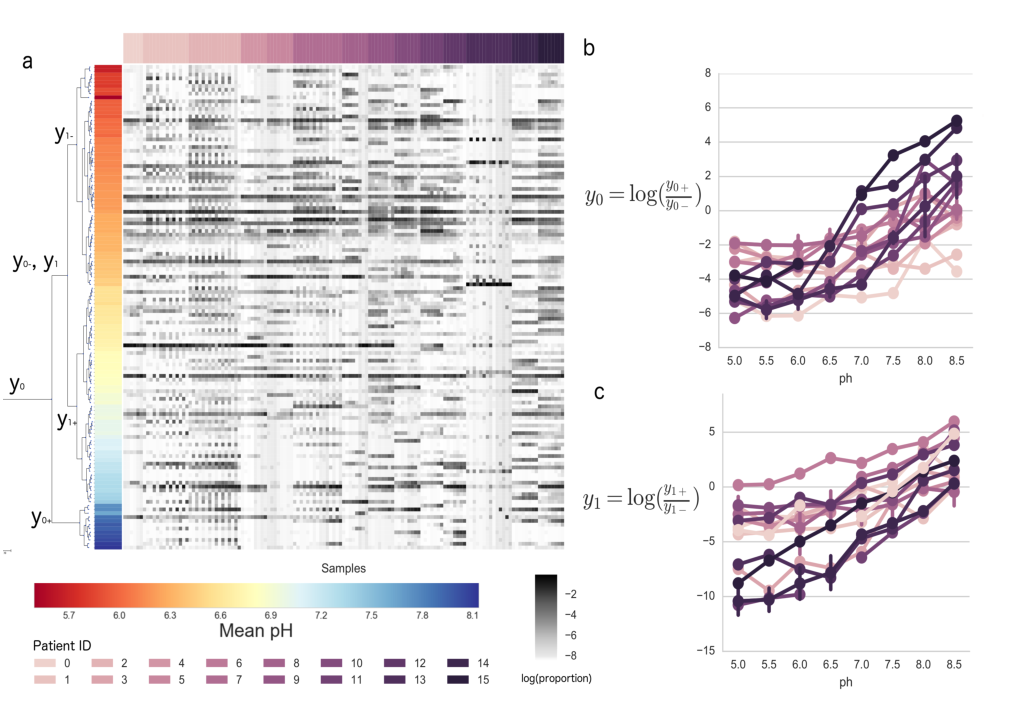
\includegraphics[width=1\textwidth]{ch3/Figure3.pdf}
        \caption[The application of balances on a cystic fibrosis dataset to identify
          microbial partitioning with respect to pH.]
        {The application of balances on a cystic fibrosis dataset to identify microbial partitioning with respect to pH.(a) A bifurcating tree generated from hierarchical clustering of \gls{otu}s based on mean pH.   The size of the internal nodes is inversely proportional to the p-value of the linear mixed effects model test on pH for that given balance.  A heatmap of all of the \gls{otu} abundances sorted by patient. \gls{otu}s were log transformed and centered across rows and columns. These abundances are aligned with the tips of the tree.  (c) The progression of the top balance over the pH for all of the patients.  (d) The progression of the second top balance over pH for all of the patients.\index{SanDiego8}}
        \label{figc3}
 \end{figure}
 A heatmap relating pH to \gls{otu} abundances across these samples does not yield clear trends (Fig 3a).  But even though we don't see a clear pattern in the heatmap, with the balance approach, we can still observe niche differentiation across the pH gradient.  In Figure \ref{figc3}b, y0 represents the log ratio of all of the high pH \gls{otu}s (7.6 $<$ mean pH $<$ 8.12) over all of the low pH \gls{otu}s (5.4 $<$ mean pH $<$ 7.4).  As the pH of the samples increases, the balance increases, likely because the low pH \gls{otu}s are becoming increasingly less abundant compared to the high pH \gls{otu}s (p-value=$7.5 \times 10^{-46}$).  The same pattern is even more apparent in y1 (Figure \ref{figc3}c). The low pH \gls{otu}s (5.4 $<$ mean pH $<$ 6.4) become increasingly less abundant than high pH \gls{otu}s (6.5 $<$ mean pH $<$ 7.4) as the sample pH increases (p-value=$2.25 x 10^{-67}$).  When Bonferroni multiple hypothesis correction was applied to these tests, the p-values were rounded down to zero.  While these patterns were not obvious when looking at the raw proportions, the balance tree approach shows very well defined trends among groups of \gls{otu}s. This can be done because even though individual \gls{otu}s may be sporadically distributed across the original samples, \gls{otu}s that thrive in similar pH niches grouped together on the environmental balance tree.  It is clear from Figure \ref{figc3}b and c that there is a transition from low pH organisms to high pH organisms along the pH gradient.  Even though the \gls{cf} patients don't have the same lung microbiomes, they contain \gls{otu}s that behave the same with respect to pH.  This pattern would not have been nearly as apparent without clustering the \gls{otu}s by mean pH and accounting for the patient effects in the linear mixed models.
 \section{ Discussion}
 In this study, we have demonstrated the benefits of applying balances to infer niche differentiation in microbes.  In the first case study, we have outlined the challenge of performing correlations of \gls{otu}s versus environmental variables, and showed how balances can capture information about species turnover across the pH gradient, which allowed us to build a model to predict microbial proportions based on pH alone.  In the second case study, we identified the challenges of studying individual \gls{otu}s due to similar niches being occupied by drastically different \gls{otu}s across different patients. Balances coupled with linear mixed models allowed us to obtain more statistically robust results, which were also more informative with respect to the differences in distribution of microbes across environmental niches.\par
 There are numerous additional benefits of analyzing species balances instead of individual species counts.  First, balances are known to be scale-invariant, so balance trees naturally correct for differences in sequencing depth without requiring rarefaction (Equation S1) and avoid many of the limitations associated with this procedure \cite{waste_not}. Second, balances are sub-compositionally coherent, which means that changes in non-overlapping sub-communities do not impact each other.  For instance, in Figures 1e and 1f, the Purple population triples and balances change because they explicitly contain the Purple species.  In contrast, the balance red and green log ratio does not change between these two scenarios because it does not relate to the Purple species (in fact, it only accounts for the Red and Green species).  This is not the case when observing the raw proportions, from which it appears as though everything is changing, even though the Purple species is the only changing species.  This phenomenon has previously been noted \cite{ancom} and can lead to extremely high false positive rates with some standard statistical techniques such as Pearson correlations or t-tests on proportions.  More discussion about this issue can be found in Figure S1. Third, arithmetic operations on balances directly translate into perturbation and powering operations on proportions \cite{ilr, Pawlowsky-Glahn2015-qb}, which can capture information about relative growth and decay of species.  This ultimately opens the door for applying standard statistical techniques, such as multiple linear regression \cite{c24} and linear mixed effects models nested design statistics directly to balances, providing additional justification for the analyses performed in the case studies.  We have shown this in the two case studies.  Finally, balances are permutation invariant.  Species can be sorted in any order deemed appropriate.  Along the same lines, these species can be rearranged into any arbitrary grouping represented as a bifurcating tree.  These trees can be built to address the questions at hand, whether it be studying species turnover across pH gradients, or even uncovering the relationships between phylogenetic clades.  In fact, balances can be thought as being utilized as an ordination technique, since every bifurcating tree forms an orthonormal basis in the Aitchison Simplex \cite{groups_of_parts}.\par
 Although the concept of balances does not address questions about properties of individual bacteria, it does answer higher-level questions concerning interactions among groups of organisms, which are arguably much more interesting from an ecological point of view. These questions can be based either on the phylogenetic tree of the bacterial community, or on environmental clustering.  There is still room for improvement on utilizing balances.  For example, the issue of zeroes still remains, because the logarithm of zero is undefined.  Currently, the common approach is to add a pseudo-count \cite{dealing_with_zeros}.  However, an appropriate tree choice can mitigate this issue, because the zeroes can be explicitly aggregated in some scenarios (Figure S2 and Figure S3).  Along the same lines, issues can arise from low-coverage samples.  If sampling is not saturated, many \gls{otu}s have low read counts, and the balances towards the tips of the trees can be highly volatile.  This is because the absolute change between one or two reads may be small for low abundance \gls{otu}s, but this will lead to large changes in log ratios, which lead to spurious signals at the tips of the tree.  As a rule of thumb, balances towards the root of the tree are more trustworthy than those at the tips of the tree.\par
 The balances approach will be key for analyzing functional roles of \gls{otu}s.  It is known that in environments like the human gut, people share very few \gls{otu}s with each other, but have roughly the same proportions of functional genes \cite{soil_pyro}.  This suggests that there is substantial functional redundancy across \gls{otu}s, which has been observed previously in time series studies in the context of infection \cite{microbiome_timeseries} — in other words, in these microbial communities many players might be sporadically distributed across similar niches.  This phenomenon could explain the sparse nature of 16S relative abundance data, and why similar environments such as human guts share few common \gls{otu}s.  Such distributions pose tremendous challenge to analyses based around identifying the niche occupancy of individual \gls{otu}s. By instead permitting the statistical comparisons to be performed across nested groups of \gls{otu}s with similar distributions, it becomes possible to robustly identify patterns of niche differentiation without requiring sufficient information be present in the abundances of each individual taxon. Identifying common functional roles of potentially diverse organisms, and analyzing the balances between these groups could significantly simplify analyses in future amplicon studies.  The ability to construct such trees would enable rapid characterizations of environmental niches, and the corresponding functional roles of the microbes occupying in these niches.\par
 All in all, balance trees are an extremely powerful tool for analyzing relative abundances and uncovering patterns associated with niche differentiation, while avoiding the issues associated with compositionality and enabling the application of conventional statistical tools.  This will ultimately open the doors for extensive mining of ecologically relevant patterns.
 \section{Methods and Materials}
 All analyses can be found in the attached IPython notebooks.  The core functions required to perform the balance basis calculations, tree visualization tools, and statistical analyses can be found in \url{https://github.com/biocore/gneiss}.  The IPython notebooks used to carry out all of the analyses can be found in the gneiss repository.  All code has been extensively unit-tested and documented. \par
 The core compositional statistics and tree data structures were are part of scikit-bio 0.4.1 and beyond. The hierarchical clustering was performed using Scipy.  Pandas and \gls{biom} \cite{biom} were used to store and manipulate the \gls{otu} tables and the metadata files.  Seaborn, matplotlib and ETE \cite{ete} were used for the visualizations.\par
 The isometric log ratio transform is an isomorphism (i.e. a function) that can map proportions to balances one to one \cite{ilr}.  These balances can be calculated as shown in Equation 1. Alternatively, they can be calculated using a linear transformation with an orthonormal basis e. This orthonormal basis can be calculated as follows
 \begin{equation}
        e_{l}=C\left [\exp(\: \: \underset{k}{\underbrace{0,...0}},\underset{r}{\underbrace{a,...a}},\underset{s}{\underbrace{b,...b}}, \underset{t}{\underbrace{0,...0}}) \right]
 \end{equation}
 \begin{equation}
        a=\frac{\sqrt{s}}{\sqrt{r(r+s)}} \quad  and \quad b=\frac{-\sqrt{r}}{\sqrt{s(r+s)}}\notag
 \end{equation}
 where $e_{l}$ refers to the balance axis aligned with the internal node \textit{l}. $C[x]$ denotes the normalization operation to normalize all of the \gls{otu} abundances to proportions that add up to 1.  $r$ refers to the number of tips in the left subtree, $s$ refers to the number of tips in the right subtree, $k$ refers to number of tips to the left of the left subtree and $t$ refers to the number of tips to the right of the right subtree. Since $e$ forms an orthonormal basis, it must have unit norm and every pair of axes in $e$ must be orthogonal.  The square root term   in Equation 1 is a normalization factor which was required for unit norm in Equation 2 (12).    Since it is not possible to take a logarithm of zero, a pseudocount of 1 was added to all of the abundance.  While this is a problem being addressed by the field, this technique is one of the more commonly used techniques \cite{dealing_with_zeros}.\par
 The mean pH used for the 2 case studies was calculated as follows.
 \begin{equation}
        \overline{g}_{x}=\sum_{i=1}^{N}g_{i}\frac{x_{i}}{\sum_{j=1}^{D}x_{j}}
 \end{equation}
 Where $x_{i}$ is the proportion of \gls{otu} \textit{x} in sample \textit{i} , $g_{x}$ is the mean pH of \gls{otu} \textit{x}, and $g_{i}$ is the sample pH at sample \textit{i}. This calculation can be found in the gneiss package under the function \textbf{mean\_niche\_estimator}. The function used to sort the tables in Figure \ref{figc2}c used \textbf{niche\_sort}. The resulting tree was built using UPGMA \cite{upgma} is shown in Figure \ref{figc2}a and Figure \ref{figc3}a, and can be generated using the scipy linkage function.\par
 This regression model is implemented in gneiss under the \textbf{ols} function.  The analysis can be found in the IPython notebooks on the gneiss repository under the ipynb folder in \textbf{88soils.ipynb}. To focus on the highest abundant organisms, only \gls{otu}s that had more than 100 reads in the entire study were considered.\par
 The linear mixed effects model is implemented in gneiss under the \textbf{mixed} functions, and the analyses can also be found in the IPython notebooks in the ipynb folder in \textbf{cfstudy.ipynb} In case study 2, only \gls{otu}s that had more than 500 reads were considered.   \par
 The Win\gls{cf} system was used according to the methods in \cite{wincf}, except only the pH dye media variable was used. The media was buffered at 0.5 units of pH from 5 to 8.5 using calculated proportions of phosphate buffer and NaOH or HCl. Sputum samples were collected from \gls{cf} patients after expectoration or induced expectoration of sputum according to the UCSD IRB approved project \#081500, and were inoculated in triplicate into capillary tubes containing the eight different pH buffered media. These eight sets of tubes in triplicate from 18 patients was then incubated at $37^{o}$C for 48 hours. The media was then removed, bacterial DNA extracted, and variable region 4 of the 16S \gls{rrna} gene was amplified and sequenced on the Illumina MiSeq platform using Earth Microbiome Project benchmarked protocols \cite{illumina_microbes, global_patterns}.  Data were processed using QIITA and \gls{otu}s were calculated using closed reference clustering at the 97\% identity cutoff for both the 88 soils and the \gls{cf} study.
\section{ Data availability}
Data for case study 1 was retrieved from Qiita (study ID 103). Data from case study 2 was retrieved from Qiita (study ID 10511).
\section{Acknowledgements}
We first acknowledge Jonathan Friedman for the original idea of applying balances to analyze microbial communities. We also acknowledge Justin Silverman and Lawrence David, in addition to Liam Toran, Tomasz Kosciolek, and Amnon Amir, for their insights and discussion on balances. In addition, we are grateful for the input from Christian Lauber and Noah Fierer concerning case study 1. Finally, we thank all of the scikit-bio developers, especially Jorge Cañardo Alastuey, Evan Bolyen, Jai Rideout, and Greg Caporaso, for reviewing the compositional statistics submodule in scikit-bio.

J.T.M. was funded by NSF grant GRFP DGE-1144086 and NSF grant IGERT 1144807 under the IQ Biology program at the University of Colorado Boulder. R.A.Q. was funded under the Cystic Fibrosis Research Innovation Award from Vertex Pharmaceuticals. This work was funded under Alfred P. Sloan Foundation grants G-2015-13933 and G-2015-13979 and National Institute of Diabetes and Digestive and Kidney Diseases (NIDDK) grant P01DK078669.

J.T.M. led the software development, benchmarking, and manuscript writing and developed the idea of applying regression to balances. J.S. contributed the idea of applying linear mixed-effects models to balances and named the software package. R.A.Q. collected the \gls{cf} lung sputum samples. D.M., A.G., J.A.N.-M., and Y.V.-B. reviewed the code in Gneiss. M.L. reviewed the mathematical notation. All authors wrote and proofread the manuscript.

Chapter 3, in full, is a reprint of the material as it appears in
``Balance Trees Reveal Microbial Niche Differentiation''
James T. Morton, Jon Sanders, Robert A. Quinn, Daniel McDonald, Antonio Gonzalez,
Yoshiki Vázquez-Baeza, Jose A. Navas-Molina, Se Jin Song, Jessica L. Metcalf,
Embriette R. Hyde, Manuel Lladser, Pieter C. Dorrestein, Rob Knight
\emph{mSystems}, 2, 2017.  The dissertation author was the primary investigator and first author of this paper.

